\chapter{The SEXTANTE graphical modeler}

\section{Introduction}

The \emph{graphical modeler} allows to create complex models using a simple and easy--to--use interface. When working with a GIS, most analysis operations are not isolated, but part of a chain of operations instead. Using the graphical modeler, that chain of processes can be wrapped into a single process, so it is easier and more convenient to execute than a single process later on a different set on inputs. No matter how many steps and different algorithms it involves, a model is executed as a single algorithm, thus saving time and effort, specially for larger models.

The modeler can be opened from the SEXTANTE menu, but also from the toolbox. In the ``Modeler'' branch of the algorithms tree you will find a group named ``tools'', which contains an entry called ``Create new model''

The modeler has a working canvas where the structure of the model and the workflow it represents are shown. On the left part of the window, a panel with two tabs can be used to add new elements to the model.

\begin{center}
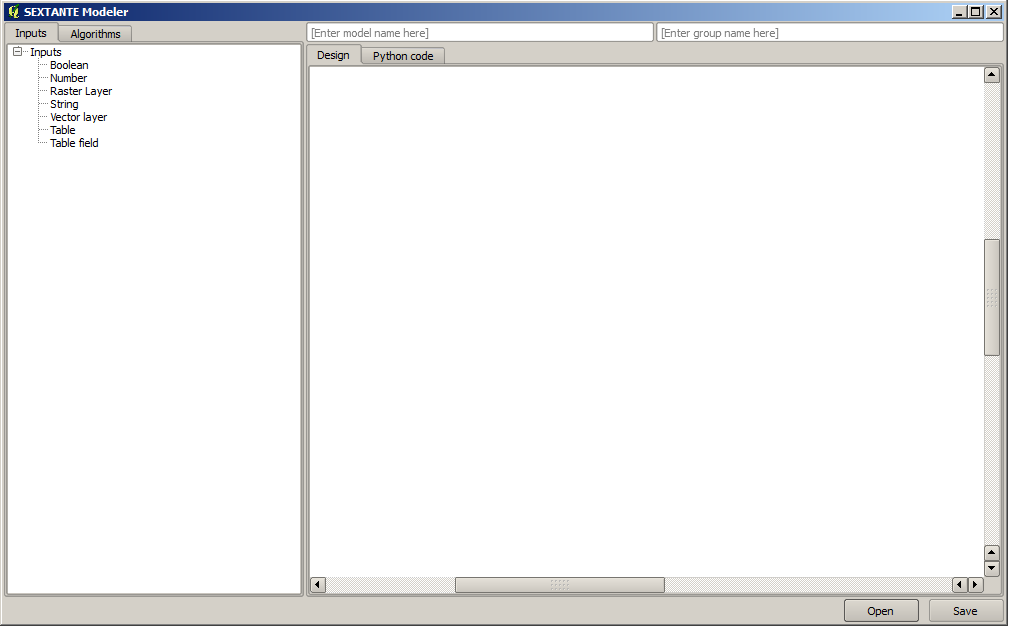
\includegraphics[width=.8\columnwidth]{modeler_canvas.png}
\end{center}

Creating a model involves two steps:

\begin{itemize}
	\item \emph{Definition of necessary inputs}. These inputs will be added to the parameters window, so the user can set their values when executing the model. The model itself is a SEXTANTE algorithm, so the parameters window is generated automatically as it happens with all the algorithms included in the library.
	\item \emph{Definition of the workflow}. Using the input data of the model, the workflow is defined adding algorithms and selecting how they use those inputs or the outputs generated by other algorithms already in the model 
\end{itemize}


\section{Definition of inputs}

The first step to create a model is to define the inputs it needs. The following elements are found in the \emph{Inputs} tabs on the left side of the modeler window:

\begin{itemize}
	\item Raster layer
	\item Vector layer 
	\item String
	\item Table field
	\item Table
	%\item Selection
	\item Numerical value 
	\item Boolean value 
\end{itemize}

Double--clicking on any of them, a dialog is shown to define its caracteristics. Depending on the parameter itself, the dialog will contain just one basic element (the description, which is what the user will see when executing the model) or more of them. For instance, when adding a numerical value, as it can be seen in the next figure, apart from the description of the parameter you have to set a default value and a range of valid values.

\begin{center}
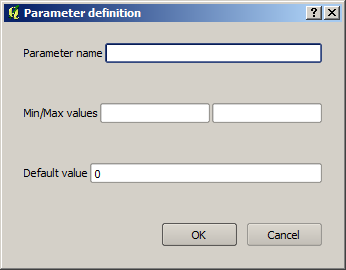
\includegraphics[width=.55\columnwidth]{models_parameters.png}
\end{center}

For each added input, a new element is added to the modeler canvas.

\begin{center}
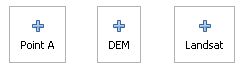
\includegraphics[width=.4\columnwidth]{models_parameters2.png}
\end{center}

\section{Definition of the workflow}

Once the inputs have been defined, it is time to define the algorithms to apply on them. Algorithms can be found in the \emph{Algorithms} tab, grouped much in the same way as they are in the toolbox.

\begin{center}
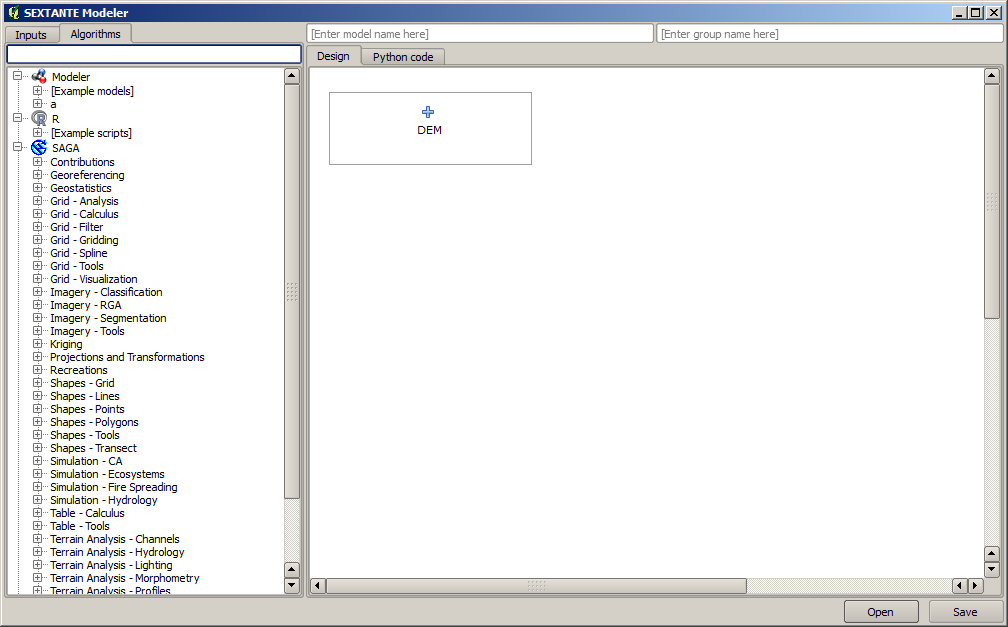
\includegraphics[width=.8\columnwidth]{models_parameters3.png}
\end{center}

To add a process, double--click on its name. An execution dialog will appear, with a content similar to the one found in the execution panel that SEXTANTE shows when executing the algorithm from the toolbox. the one shown next correspond to the SAGA convergence index algorithm, the same one we saw in the chapter dedicated to the SEXTANTe toolbox.

\begin{center}
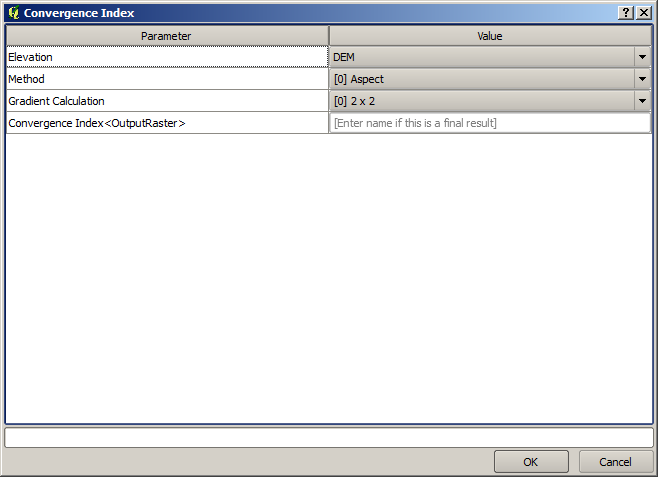
\includegraphics[width=.8\columnwidth]{models_parameters4.png}
\end{center}

as you can see, some differences exist. Instead of the file output box that was used to set the filepath for output layers and tables, a simple text box is. If the layer generated by the algorithm is just a temporary result that will be used as the input of another algorithm and should not be kept as a final result, just do not edit that textbox. Typing anything on it means that the result is a final one, and the text that you supply will be the description for the output, which will be the one the user will see when executing the model. 

Selecting the value of each parameter is also a bit different, since there are importante differences between the context of the modeler and the toolbox one. Let's see how to introduce the values for each type of parameter.
\begin{itemize}
	\item Layers (raster and vector) and tables. They are selectend from a list, but in this case the possible values are not the layers or tables currently loaded in QGIS, but the list of model inputs of the corresponding type, or other layers or tables generated by algorithms already added to the model.
	\item Numerical values. Literal values can be introduced directly on the textbox. But this textbox is also a list that can be used to select any of the numerical value inputs of the model. In this case, the parameter will take the value introduced by the user when executing the model. 
	\item String. Like in the case of numerical values, literal strings can be typed, or an input string can be selected.
	\item Table field. The fields of the parent table or layer cannot be known at design--time, since they depend of the selection of the user each time the model is executed. To set the value for this parameter, type the name of a field directly in the textbox, or use the list to select a table field input already added to the model. The validity of the selected field will be checked by SEXTANTE at run--time
	%\item Selection. The list contains in this case not only the available option from the algorithm, but also the selection inputs already added to the current model
\end{itemize}

Once all the parameter have been assigned valid values, click on \emph{OK} and the algorithm will be added to the canvas. It will be linked to all the other elements in the canvas, whether algorithms or inputs, which provide objects that are used as inputs for that algorithm.

\begin{center}
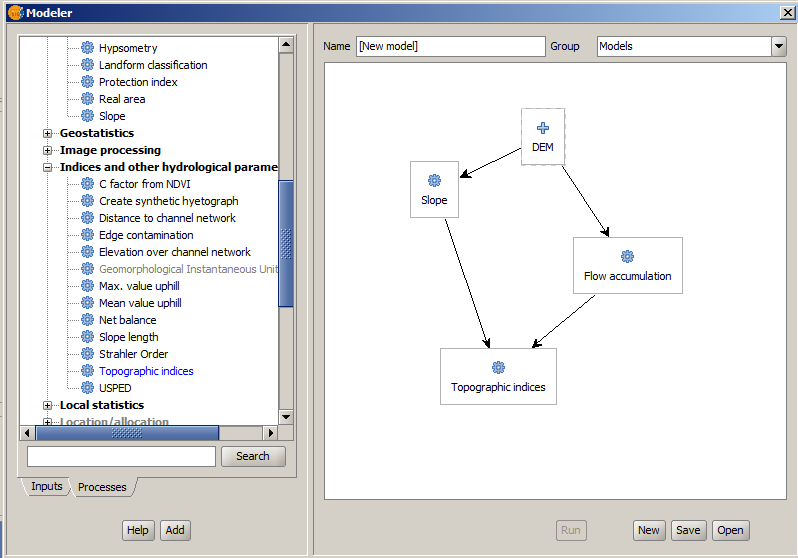
\includegraphics[width=.8\columnwidth]{models_parameters5.png}
\end{center}


%\section{Editing the model}
%
%Once the model has been designed, it can be executed clicling on the \emph{Execute} button. The execution window will have a parameters tab automatically created based on the requirements of the model (the inputs added to it), just like it happens when a simple algorithm is executed. If any of the algorithms of the model generates raster layers, the \emph{Raster output} tab will be added to the window. 
%
%Elements can be dragged to a different position within the canvas, to change the way the module structure is displayed and make it more clear and intuitive. Links between elements are update automatically.
%
%To change the parameters of any of the algorithms of a model, double--click on it to acces its parameters window.
%
%To delete an element, right--click on it and select \emph{Delete}. Only those elements that do not have any other one depending on them can be deleted. If you try to delete an element that cannot be deleted, SEXTANTE will show the following warning message.


\section{Saving and loading models}


Use the \emph{Save} button to save the current model and the \emph{Open} one to open any model previously saved. Model are saved with the \texttt{.model} extension. If the model has been previously saved from the modeler window, you will not be prompted for a filename, since there is already a file associated with that model, and it will be used.

Before saving a model, you have to enter a name and a group for it, using the text boxes in the upper part of the window.

Models saved on the models folder (the default folder when you are prompted for a filename to save the model) will appear in the toolbox in the corresponding branch. When the toolbox is invoked, SEXTANTE searches the models folder for files with \texttt{.model} extension and loads the models they contain. Since a model is itself a SEXTANTE algorithm, it can be added to the toolbox just like any other algorithm.

The models folder can be set from the SEXTANTE configuration dialog, under the ``Modeler'' group.

Models loaded from the models folder appear not only in the toolbox, but also in the algorithms tree in the \emph{Algorithms} tab of the modeler window. That means that you can incorporate a model as a part of a bigger model, just as you add any other algorithm. 

\begin{center}
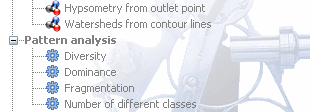
\includegraphics[width=.5\columnwidth]{models_icon.png}
\end{center}

%By default, the models folder is the same one as the folder where SEXTANTE help files are located. This folder contains a small set of example models, that you can use to better understand how the modeler works. Open them and study how they are constructed. You can also check their associated help files. As it has been said, models are themselves SEXTANTE algorithms, so they can have their own help files, and these can be edited as we have already seen in the previous chapter.